\section{Конструкторская часть}

\subsection{IDEF0}
\begin{figure}[h]
	\begin{center}
		{\includegraphics[scale = 0.3]{img/idef0/main.png}}
		\caption{Анализ входных и выходных данных}
		\label{fig29:image}
	\end{center}
\end{figure}

%\newpage

\begin{figure}[h!]
	\begin{center}
		{\includegraphics[scale = 0.3]{img/idef0/down.png}}
		\caption{Последовательность преобразований}
		\label{fig200:image}
	\end{center}
\end{figure}

\newpage

\subsection{Поддерживаемые возможности межсетевого экрана}
В соответствии с параграфом \ref{sec:task} межсетевой экран должен предоставлять следующие возможности:
\begin{itemize}
	\item добавление нового правила;

	\item удаление правила;
	
	\item просмотр всех правил;
	
	\item сокрытие модуля в системе;
	
	\item обнаружение модуля в системе. \\
\end{itemize}

Для непосредственного взаимодействия с пользователем необходимо разработать отдельную программу, представляющую из себя интерфейс для работы с загружаемым модулем. Программа выполняет не только функцию связующего звена между пользователем и межсетевым экраном, но и проверку входных данных: корректность вводимых команд и правил. \newline

\subsection{Структура программного обеспечения}
Составляющие проекта приведены на Рисунке \ref{fig30:image}.
\begin{figure}[h!]
	\begin{center}
		{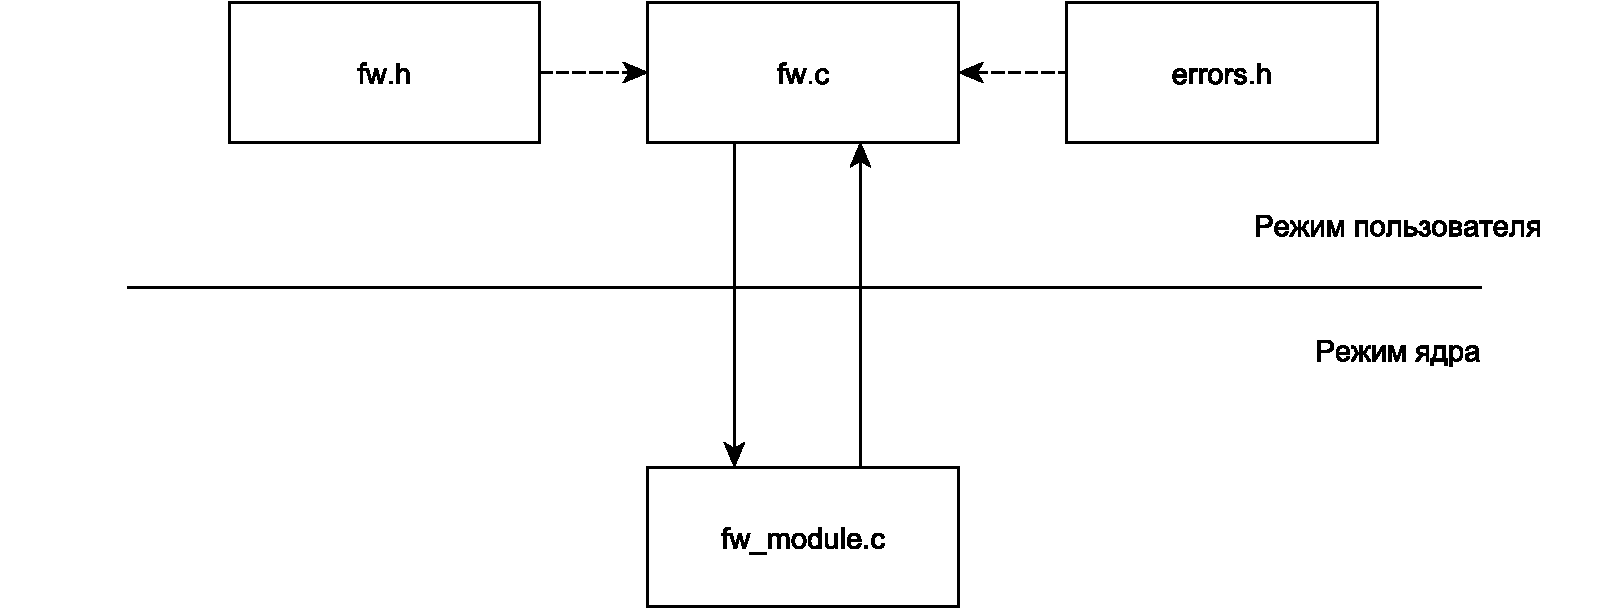
\includegraphics[scale = 0.63]{img/struct.pdf}}
		\caption{Структура ПО}
		\label{fig30:image}
	\end{center}
\end{figure}

\subsection{Алгоритм инициализации межсетевого экрана}
На Рисунке \ref{fig21:image} представлен алгоритм инициализации межсетевого экрана.
\begin{figure}[h!]
	\begin{center}
		{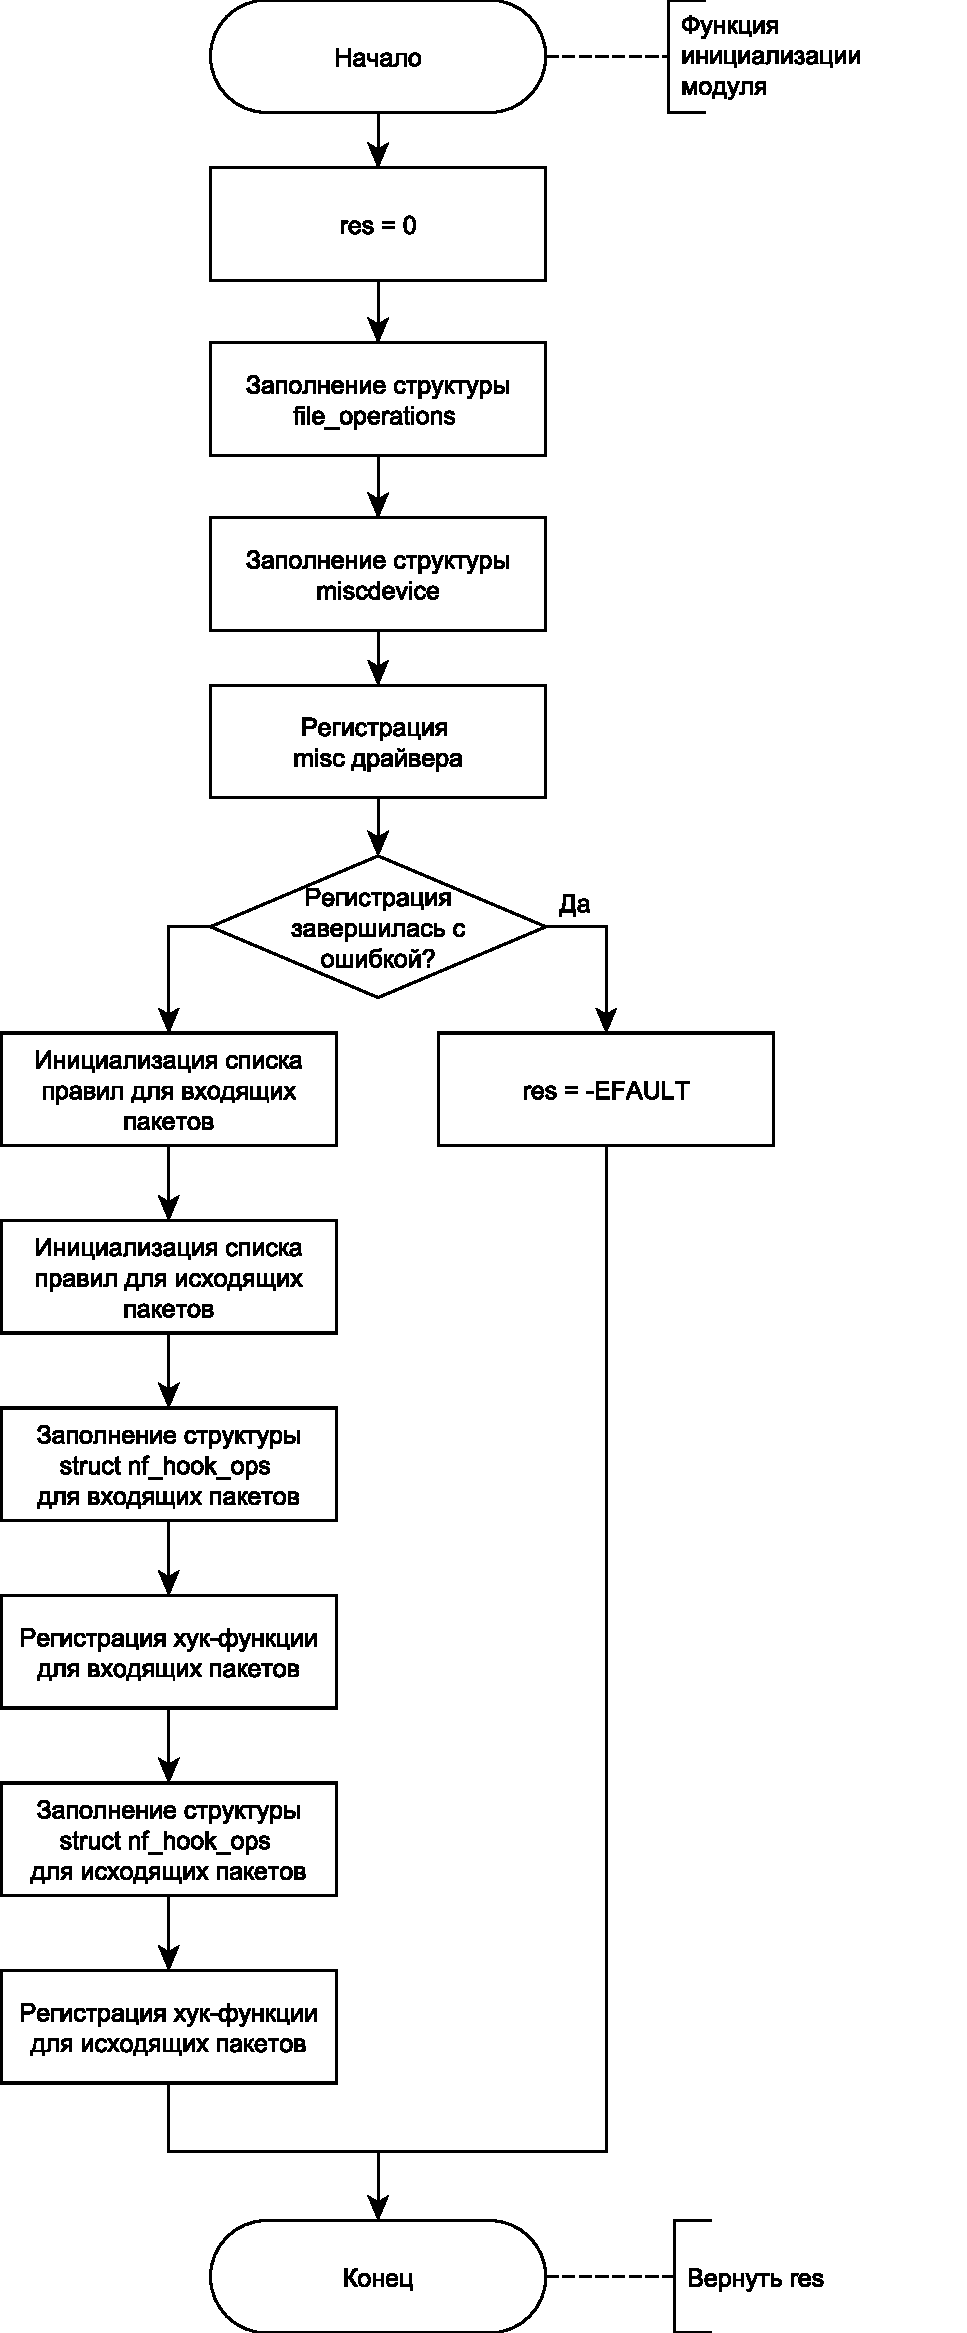
\includegraphics[scale = 0.57]{img/init.pdf}}
		\caption{Алгоритм инициализации межсетевого экрана}
		\label{fig21:image}
	\end{center}
\end{figure}

\newpage

\subsection{Алгоритм завершения работы межсетевого экрана}
При выгрузке необходимо освободить все ресурсы, которые были зарезервированы. Детально алгоритм завершения работы межсетевого экрана изложен на Рисунке \ref{fig22:image}.
\begin{figure}[h!]
	\begin{center}
		{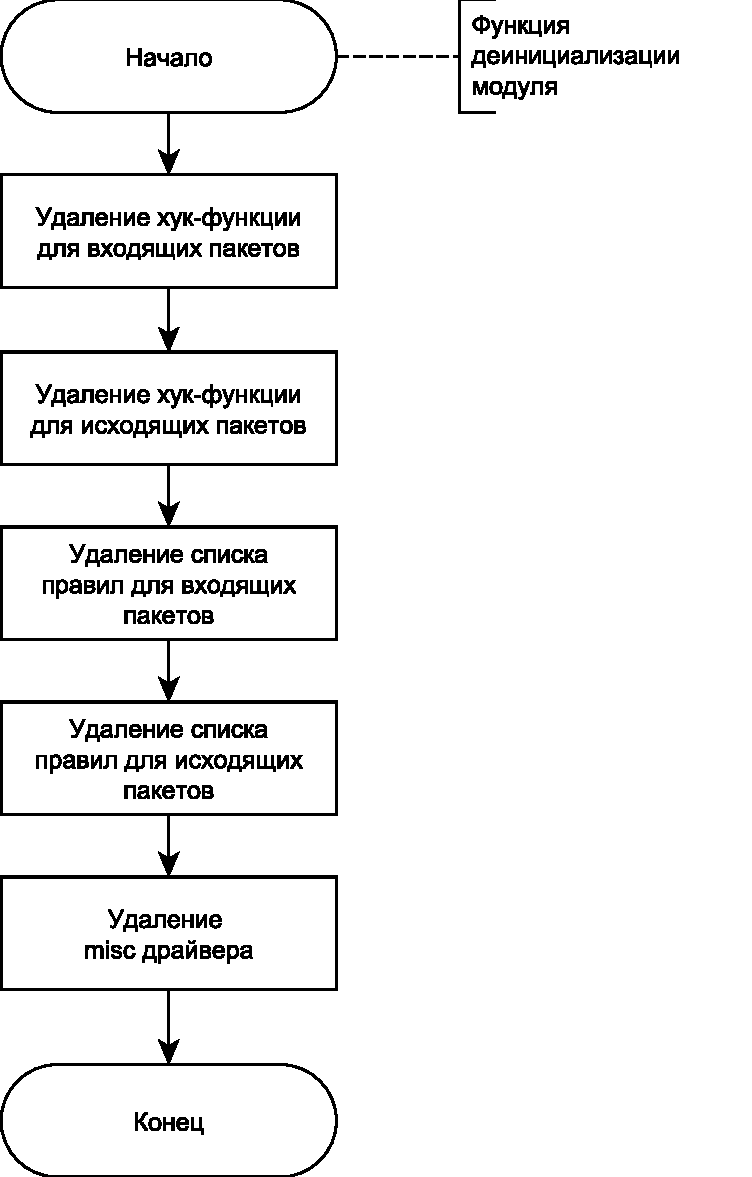
\includegraphics[scale = 0.6]{img/exit.pdf}}
		\caption{Алгоритм завершения работы межсетевого экрана}
		\label{fig22:image}
	\end{center}
\end{figure}

\newpage

\subsection{Алгоритм чтения правил межсетевого экрана}
На Рисунке \ref{fig23:image} приведен алгоритм чтения правил.
\begin{figure}[h!]
	\begin{center}
		{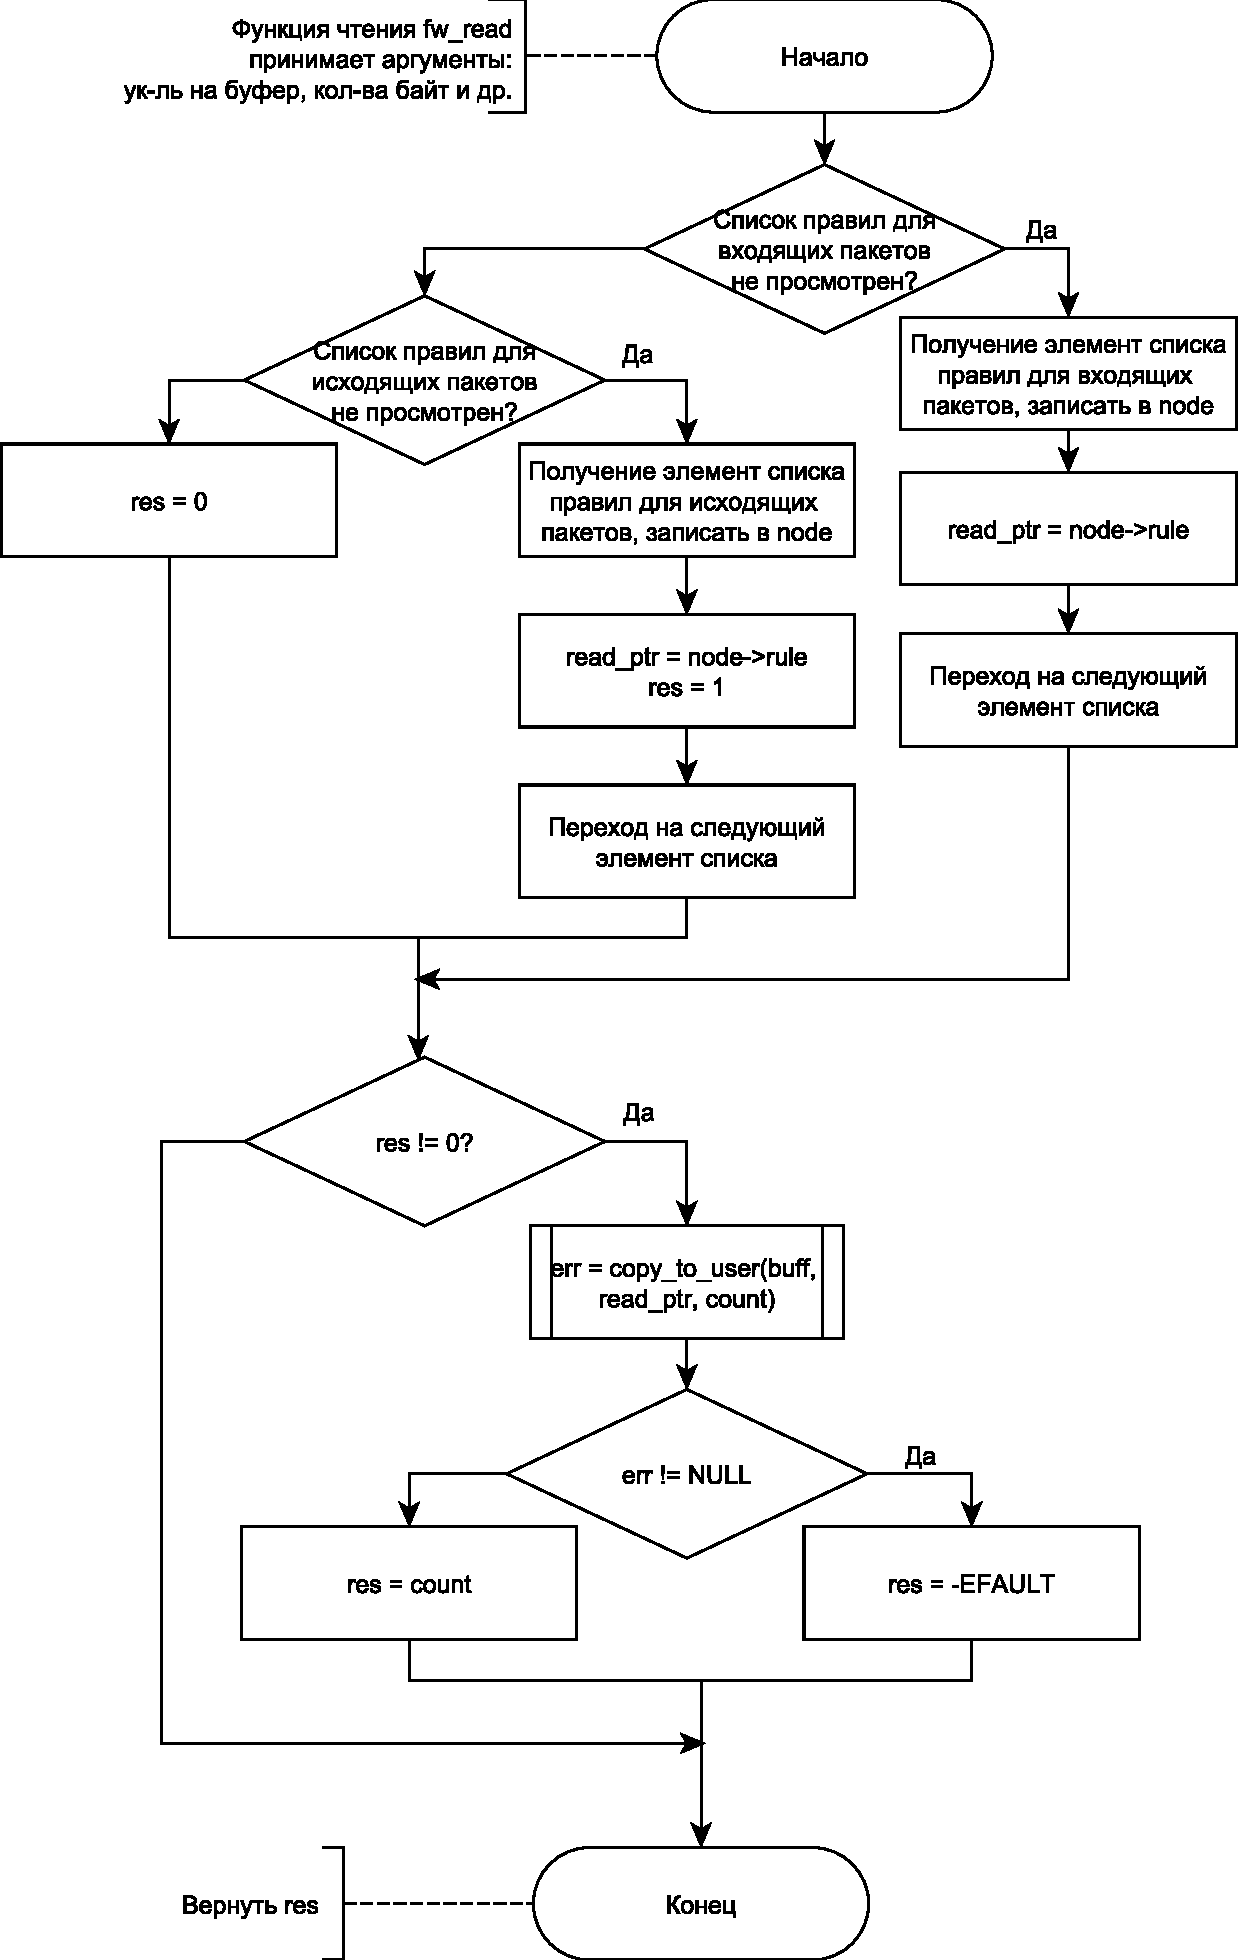
\includegraphics[scale = 0.63]{img/read.pdf}}
		\caption{Алгоритм чтения правил}
		\label{fig23:image}
	\end{center}
\end{figure}

\newpage

\subsection{Алгоритм обработки запроса}
На Рисунке \ref{fig24:image} приведен алгоритм обработки пользовательского запроса.
\begin{figure}[h!]
	\begin{center}
		{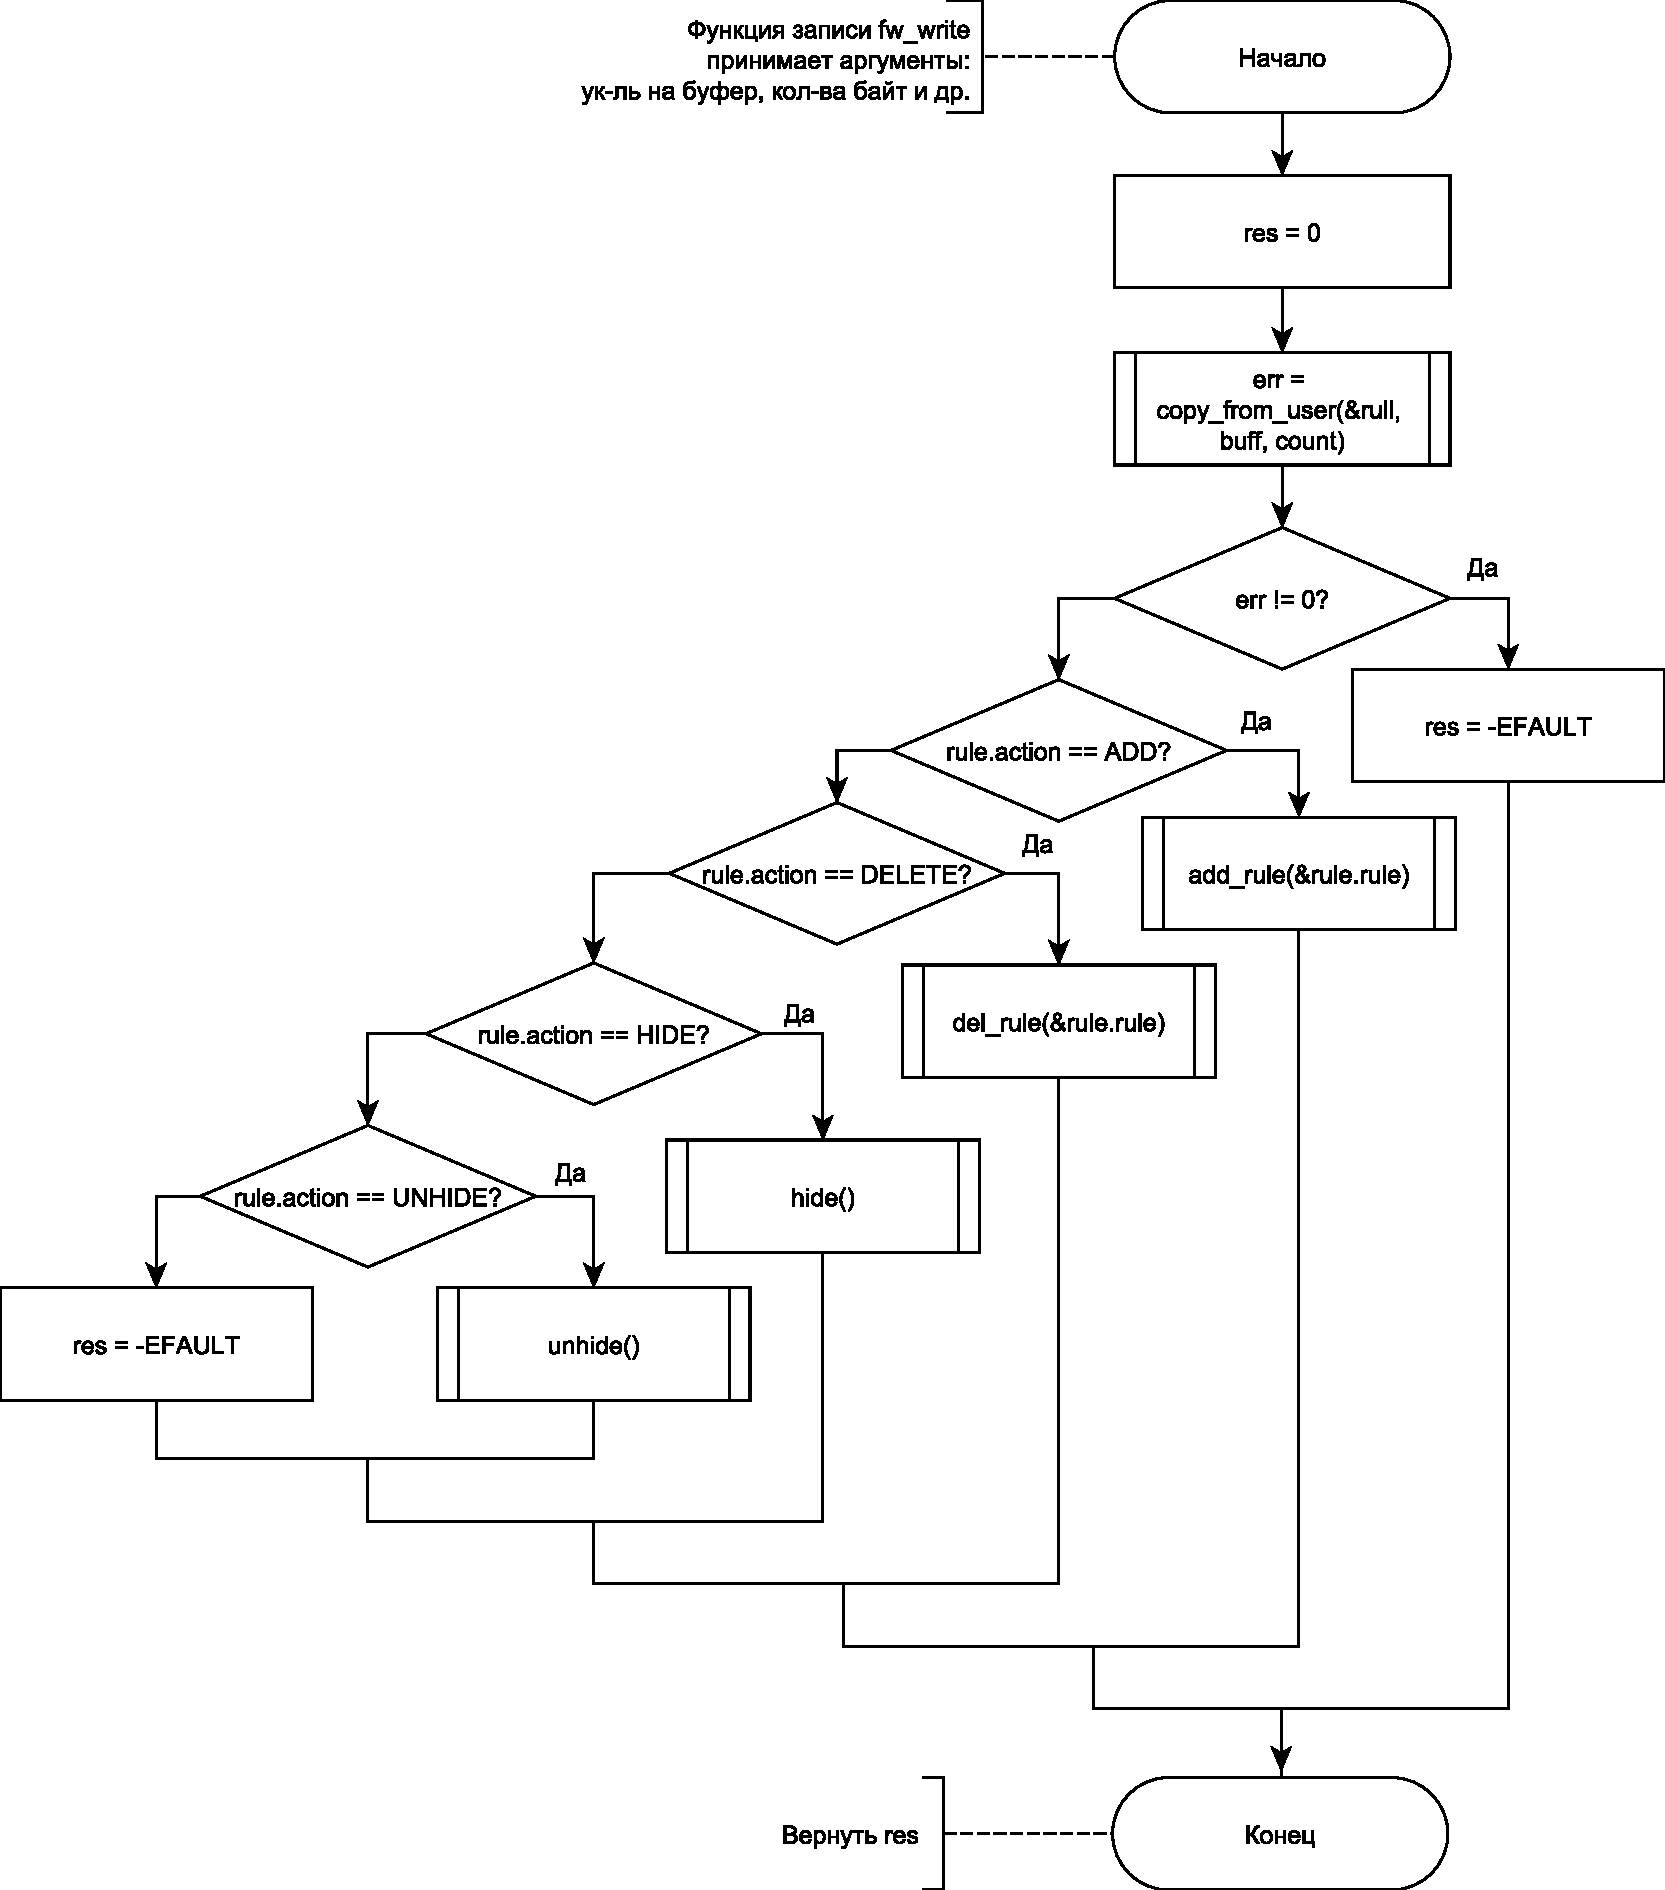
\includegraphics[scale = 0.6]{img/write.pdf}}
		\caption{Алгоритм обработки запроса}
		\label{fig24:image}
	\end{center}
\end{figure}

\newpage

\subsection{Алгоритм добавления правил}
Пользователю предоставляется возможность добавить новое правило. На Рисунке \ref{fig25:image} показан общий подход к реализации этой возможности.

\begin{figure}[h!]
	\begin{center}
		{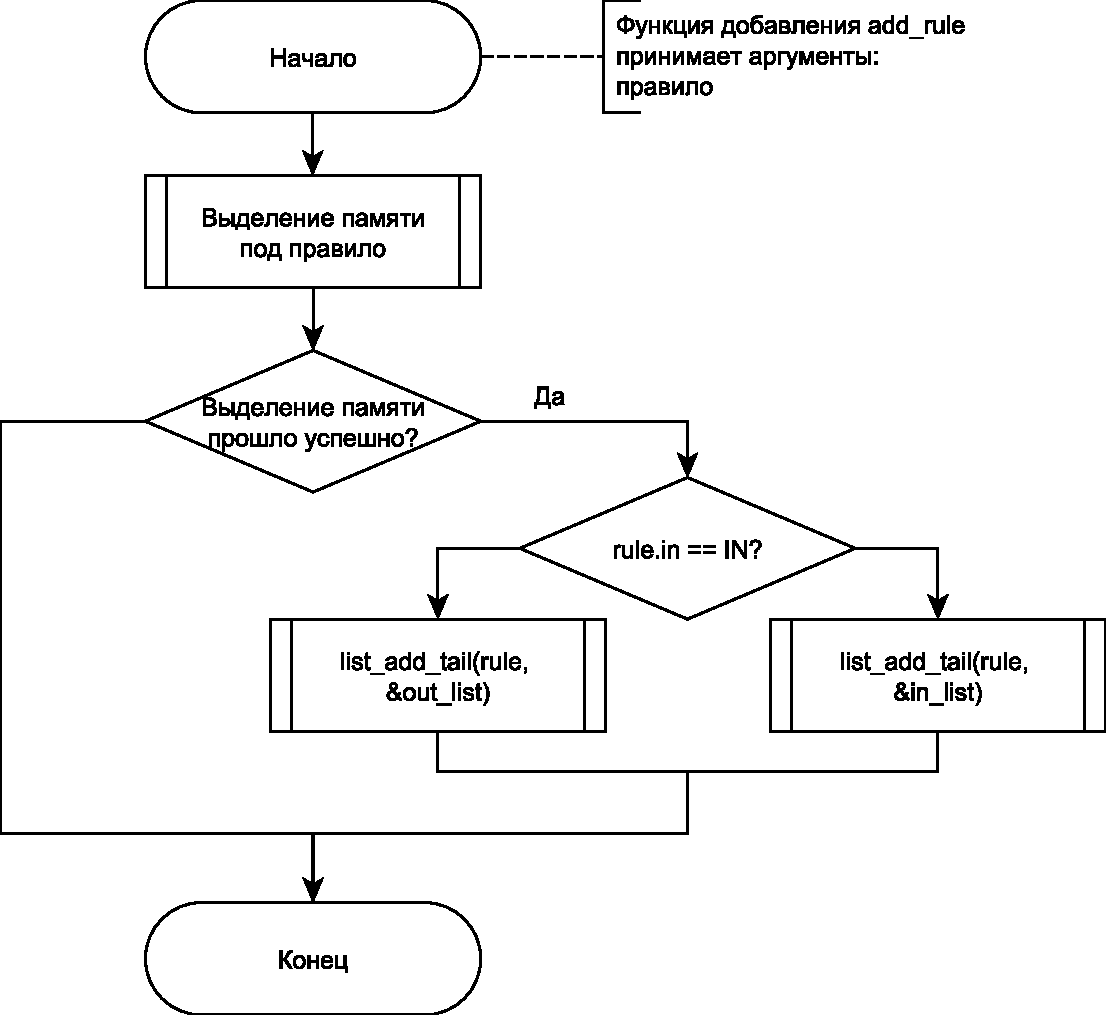
\includegraphics[scale = 0.6]{img/add_rule.pdf}}
		\caption{Алгоритм добавления нового правила}
		\label{fig25:image}
	\end{center}
\end{figure}

\newpage

\subsection{Алгоритм удаления правила}
Пользователь также может удалить уже существующее правило. На Рисунке \ref{fig26:image} приведена соответствующая схема.

\begin{figure}[h!]
	\begin{center}
		{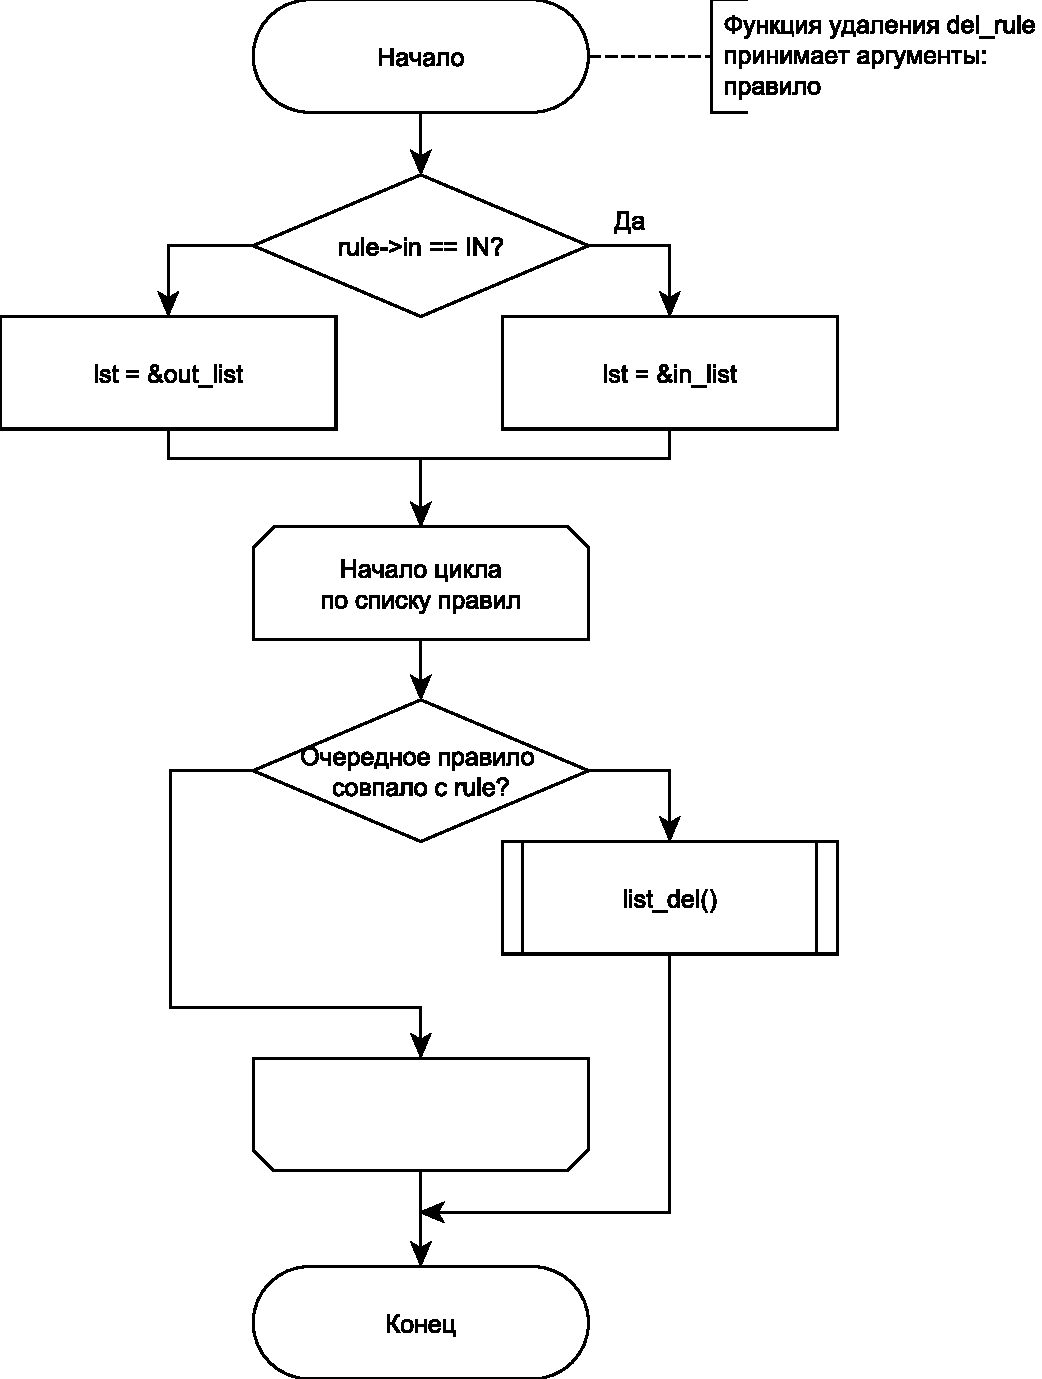
\includegraphics[scale = 0.55]{img/del_rule.pdf}}
		\caption{Алгоритм удаления правила}
		\label{fig26:image}
	\end{center}
\end{figure}

\pagebreak

\subsection{Алгоритм фильтрации пакетов}\label{sec:filter}
В процессе инициализации также происходит регистрация хук-функций, заданных в структуре \textbf{struct nf\_hook\_ops}. 

В рамках поставленной задачи регистрируются две функции: для обработки входящих и исходящих пакетов. Поскольку главное их отличие -- направление анализируемых единиц, то рекомендуется реализовать одну функцию, в которую подаётся соответствующий список правил. Детали представлены на Рисунках \ref{fig27:image} -- \ref{fig28:image}.

\begin{figure}[h!]
	\begin{center}
		{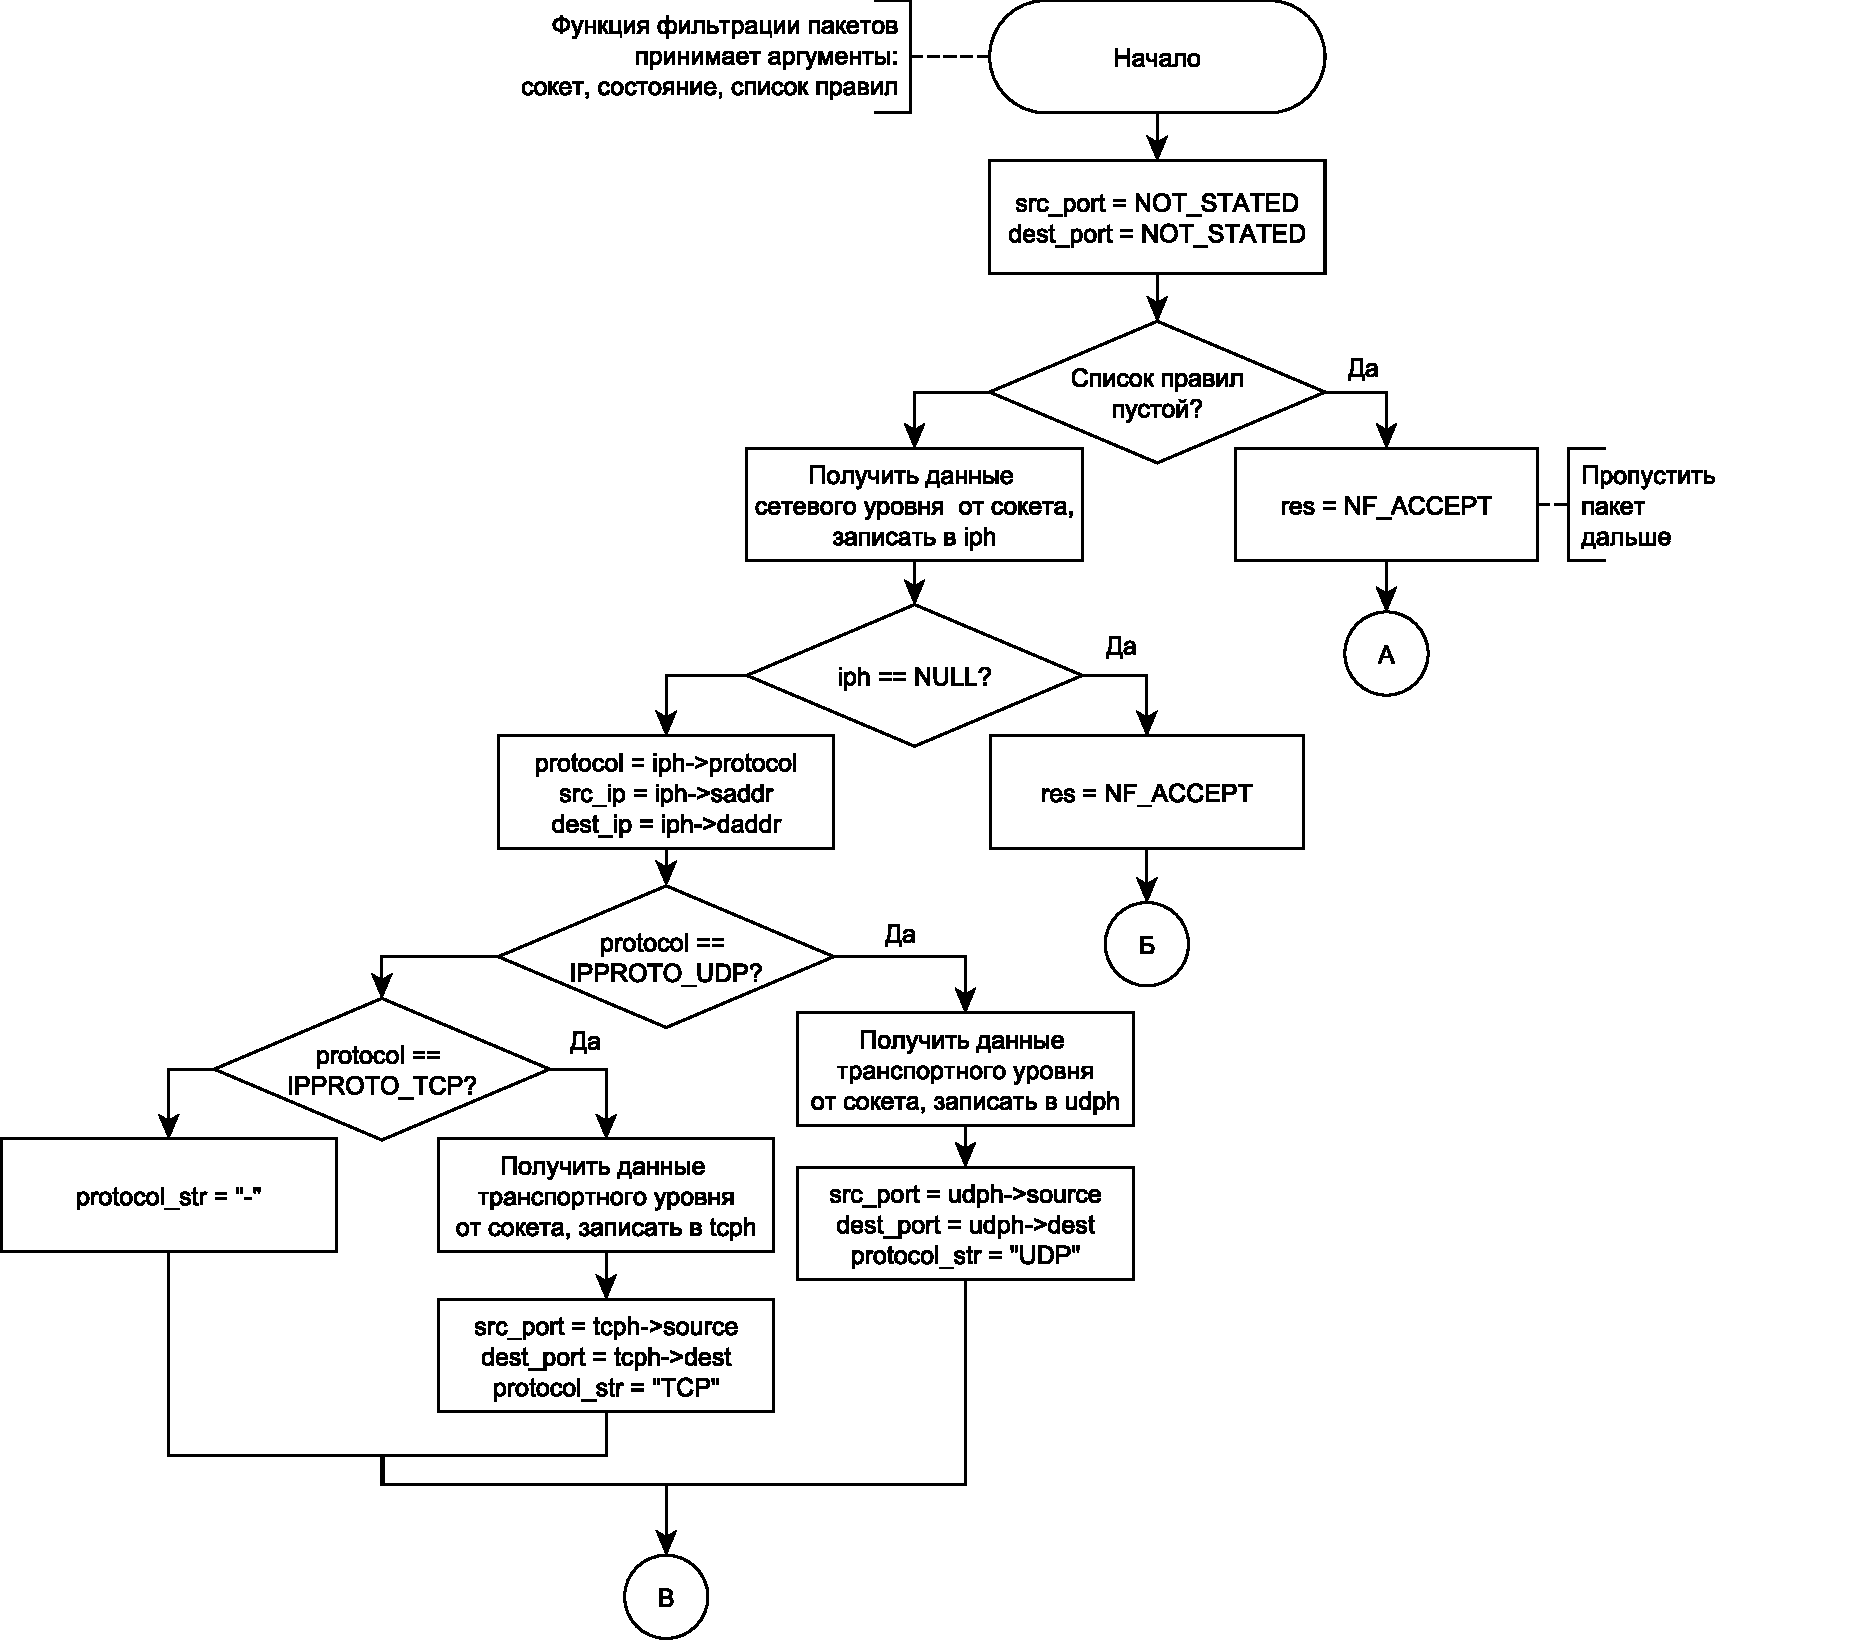
\includegraphics[scale = 0.56]{img/filter1.pdf}}
		\caption{Алгоритм фильтрации пакетов}
		\label{fig27:image}
	\end{center}
\end{figure}

\begin{figure}[h!]
	\begin{center}
		{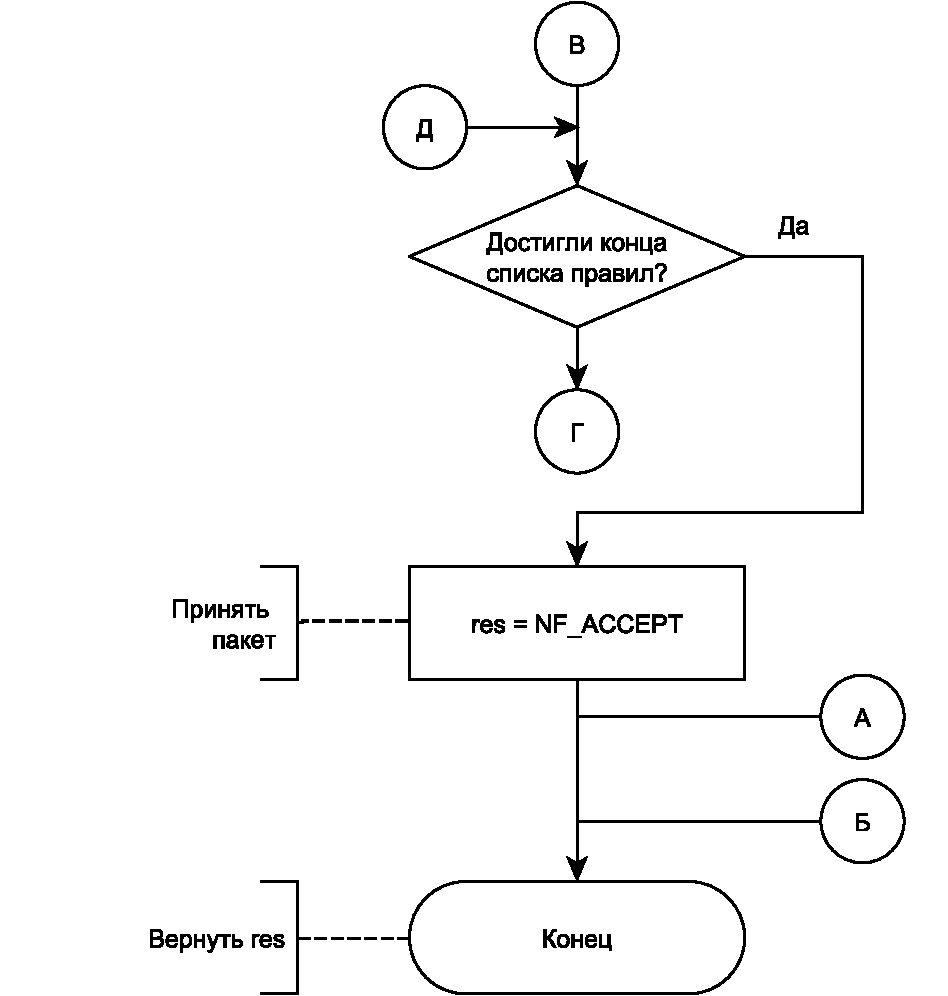
\includegraphics[scale = 0.56]{img/filter2.pdf}}
		\caption{Алгоритм фильтрации пакетов}
		\label{fig28:image}
	\end{center}
\end{figure}
